% ==================///==================///==================///
% ==================/// LATEX'S STUFF
% ==================///==================///==================///

\documentclass[hungarian]{beamer}
\usepackage[T1]{fontenc}
\usepackage{babel}
\usepackage{graphicx}
\usepackage{hyperref}
\usepackage{stuki}

\usepackage{soul}

\usepackage{tikz}
\usetikzlibrary{shapes.multipart, positioning, arrows.meta}
\tikzset{list/.style={rectangle multipart, draw, minimum height=1cm, minimum width=1.5cm}}

\usepackage{amsfonts,amsmath,oldgerm}
\usetheme{_statale}
\usefonttheme[onlymath]{serif}

\newcommand{\testcolor}[1]{\colorbox{#1}{\textcolor{#1}{test}}~\texttt{#1}}
\newcommand{\hrefcol}[2]{\textcolor{cyan}{\href{#1}{#2}}}
\titlebackground*{assets/background}

\newcommand{\Ord}{\mathcal{O}}

\newcommand{\CtwoL}[1]{%
\begin{tikzpicture}[
    list/.style={
        rectangle split,
        rectangle split parts=3,
        draw,
        rectangle split horizontal,
        minimum height=0.8cm,
        inner sep=6pt,
        fill=blue!5
    },
    pointer/.style={
        -Stealth,
        thick
    },
    transform canvas={scale=#1}
]

    % Head pointer label
    \node (head) {\textbf{L}};

    % Nodes
    \node[list, right=0.8cm of head, fill=blue!20] (node0) {\nodepart{two} \nodepart{three}};
    \node[list, right=1.2cm of node0] (node1) {\nodepart{two} 11 \nodepart{three}};
    \node[list, right=1.2cm of node1] (node2) {\nodepart{two} 79 \nodepart{three}};
    \node[list, right=1.2cm of node2] (node3) {\nodepart{two} 43 \nodepart{three}};

    % Arrows / Pointers
    \draw[pointer] (head.east) ++(0.1,0) -- (node0);

    \draw[pointer] (node0.east) ++(-0.3,0.1) -- ([yshift=0.1cm]node1.west);
    \draw[pointer] (node1.east) ++(-0.3,0.1) -- ([yshift=0.1cm]node2.west);
    \draw[pointer] (node2.east) ++(-0.3,0.1) -- ([yshift=0.1cm]node3.west);
    \draw[pointer] (node3.east) ++(-0.3,0.1) -- ++(0,0.7) -- ([yshift=0.4cm]node0.north) -- (node0.north);

    \draw[pointer] (node1.west) ++(0.3,-0.1) -- ([yshift=-0.1cm]node0.east);
    \draw[pointer] (node2.west) ++(0.3,-0.1) -- ([yshift=-0.1cm]node1.east);
    \draw[pointer] (node3.west) ++(0.3,-0.1) -- ([yshift=-0.1cm]node2.east);
    \draw[pointer] (node0.west) ++(0.3,-0.1) -- ++(0,-0.7) -- ([yshift=-0.4cm]node3.south) -- (node3.south);

\end{tikzpicture}
}


% ==================///==================///==================///
% ==================/// SPLASH PAGE
% ==================///==================///==================///

\title{Algoritmusok I.}
\newcommand{\longauthor}{4. gyakorlat}
\author{Sipos Ágoston}
\newcommand{\correspondingauthor}{John Doe}
\newcommand{\email}{siposagoston@inf.elte.hu}
\renewcommand{\insertdate}{2026. szeptember 30.}

% ==================///==================///==================///
% ==================/// START PRESENTATION
% ==================///==================///==================///

\begin{document}
\maketitle

\section{Fejelemes lista}

\begin{frame}{Fejelemes egyirányú lista (H1L)}

Ötlet: legyen egy fix elem a lista elején, ami nem tartalmaz értéket / kulcsot.

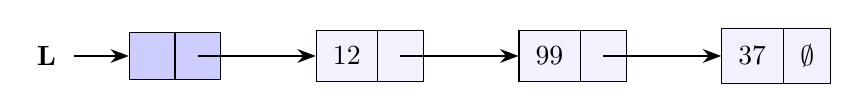
\begin{tikzpicture}[
    list/.style={
        rectangle split,
        rectangle split parts=2,
        draw,
        rectangle split horizontal,
        minimum height=0.6cm,
        inner sep=6pt,
        fill=blue!5
    },
    pointer/.style={
        -Stealth,
        thick
    }
]

    % Head pointer label
    \node (head) {\textbf{L}};

    % Nodes
    \node[list, right=0.8cm of head, fill=blue!20] (node0) { \nodepart{two}};
    \node[list, right=1.2cm of node0] (node1) {12 \nodepart{two}};
    \node[list, right=1.2cm of node1] (node2) {99 \nodepart{two}};
    \node[list, right=1.2cm of node2] (node3) {37 \nodepart{two} $\emptyset$};

    % Arrows / Pointers
    \draw[pointer] (head.east) ++(0.1,0) -- (node0);
    \draw[pointer] (node0.east) ++(-0.3,0) -- (node1.west);
    \draw[pointer] (node1.east) ++(-0.3,0) -- (node2.west);
    \draw[pointer] (node2.east) ++(-0.3,0) -- (node3.west);

\end{tikzpicture}

Egyszerűsíti a beszúrás, törlés algoritmusát: sosem kell a lista kezdetére mutató mutatót állítani, mindig ugyanazok a lépések.

Beszúrás (p elem mögé, p mutathat a fejelemre is):

\setlength{\stukiwidth}{4cm}
\begin{stukibox}
\stm*{q = new E1}
\stm*{q->key = k}
\stm*{q->next = p->next}
\stm*{p->next = q}
\end{stukibox}

Törlés hasonlóan.
    
\end{frame}

\section{Kétirányú lista}

\begin{frame}{Egyszerű kétirányú lista (E2L)}

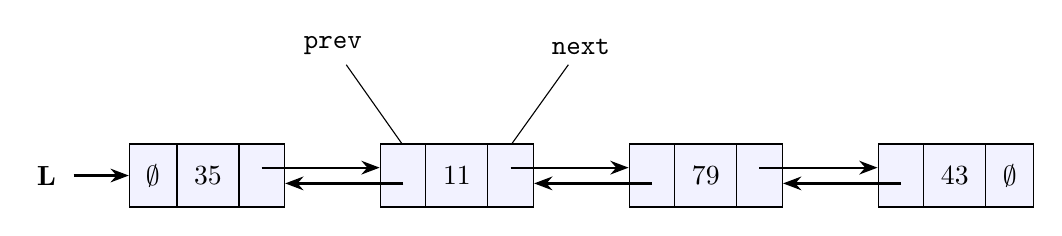
\begin{tikzpicture}[
    list/.style={
        rectangle split,
        rectangle split parts=3,
        draw,
        rectangle split horizontal,
        minimum height=0.8cm,
        inner sep=6pt,
        fill=blue!5
    },
    pointer/.style={
        -Stealth,
        thick
    }
]

    % Head pointer label
    \node (head) {\textbf{L}};

    % Nodes
    \node[list, right=0.8cm of head] (node0) {$\emptyset$ \nodepart{two} 35 \nodepart{three}};
    \node[list, right=1.2cm of node0] (node1) {\nodepart{two} 11 \nodepart{three}};
    \node[list, right=1.2cm of node1] (node2) {\nodepart{two} 79 \nodepart{three}};
    \node[list, right=1.2cm of node2] (node3) {\nodepart{two} 43 \nodepart{three} $\emptyset$};

    
    \node[above left=1cm and 0.1cm of node1] (prev) {\texttt{prev}};
    \node[above right=1cm and 0.1cm of node1] (next) {\texttt{next}};

    % Arrows / Pointers
    \draw[pointer] (head.east) ++(0.1,0) -- (node0);

    \draw[pointer] (node0.east) ++(-0.3,0.1) -- ([yshift=0.1cm]node1.west);
    \draw[pointer] (node1.east) ++(-0.3,0.1) -- ([yshift=0.1cm]node2.west);
    \draw[pointer] (node2.east) ++(-0.3,0.1) -- ([yshift=0.1cm]node3.west);

    \draw[pointer] (node1.west) ++(0.3,-0.1) -- ([yshift=-0.1cm]node0.east);
    \draw[pointer] (node2.west) ++(0.3,-0.1) -- ([yshift=-0.1cm]node1.east);
    \draw[pointer] (node3.west) ++(0.3,-0.1) -- ([yshift=-0.1cm]node2.east);

    \draw (prev) -- ([xshift=-0.7cm]node1.north);
    \draw (next) -- ([xshift=0.7cm]node1.north);

\end{tikzpicture}

\begin{itemize}
    \item Könnyebb benne mozogni, mint az egyirányú listában.
    \item Nem kell előző elemre való mutatót tárolni.
    \item Nem fejelemes: az első elem kezelése speciális logikát igényel.
    \item Beszúrásnál, törlésnél több mutatót kell állítani.
    \item Nagyobb memóriaigény.
\end{itemize}

Lehet H2L, a H1L-hez analóg módon
    
\end{frame}

\begin{frame}{Fejelemes, ciklikus kétirányú lista (C2L)}

\vspace*{5mm}

\CtwoL{1}

\vspace{1cm}

\begin{itemize}
    \item Minden elem tartalmazza az előző, és a következő mutatót
    \item Az utolsó elem \texttt{next}-je a fejelemre mutat, a fejelem \texttt{prev}-je az utolsó elemre
    \item Tehát a bejárás addig tart, amíg visszaérünk a fejelemhez\pause
    \item Üres lista: egyetlen fejelem, a mutatói önmagára mutatnak (nincs NULL)
\end{itemize}

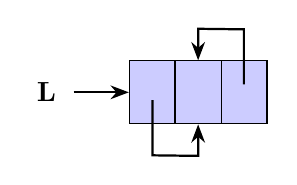
\begin{tikzpicture}[
    list/.style={
        rectangle split,
        rectangle split parts=3,
        draw,
        rectangle split horizontal,
        minimum height=0.8cm,
        inner sep=6pt,
        fill=blue!5
    },
    pointer/.style={
        -Stealth,
        thick
    }
]

    % Head pointer label
    \node (head) {\textbf{L}};

    % Nodes
    \node[list, right=0.8cm of head, fill=blue!20] (node0) {\nodepart{two} \nodepart{three}};

    % Arrows / Pointers
    \draw[pointer] (head.east) ++(0.1,0) -- (node0);

    \draw[pointer] (node0.east) ++(-0.3,0.1) -- ++(0,0.7) -- ([yshift=0.4cm]node0.north) -- (node0.north);

    \draw[pointer] (node0.west) ++(0.3,-0.1) -- ++(0,-0.7) -- ([yshift=-0.4cm]node0.south) -- (node0.south);

\end{tikzpicture}

\end{frame}

\begin{frame}{C2L beszúró, törlő műveletek}

\begin{columns}

\begin{column}{0.4\linewidth}

\only<1>{

Beszúrás adott elem elé:

\vspace{5mm}

\setlength{\stukiwidth}{4cm}
\begin{stukibox*}{precede(r : E2*)}
\stm*{p = r->prev}
\stm*{q = new E1}
\stm*{q->key = k}
\stm*{q->next = r}
\stm*{r->prev = q}
\stm*{q->prev = p}
\stm*{p->next = q}
\end{stukibox*}

}

\only<2>{

Beszúrás adott elem mögé:

\vspace{5mm}

\setlength{\stukiwidth}{4cm}
\begin{stukibox*}{follow(p : E2*)}
\stm*{r = p->next}
\stm*{q = new E1}
\stm*{q->key = k}
\stm*{q->next = r}
\stm*{r->prev = q}
\stm*{q->prev = p}
\stm*{p->next = q}
\end{stukibox*}

}

\only<3>{

Adott elem kiláncolása a listából:

\vspace{2mm}

\setlength{\stukiwidth}{4cm}
\begin{stukibox*}{unlink(q : E2*)}
\stm*{p = q->prev}
\stm*{r = q->next}
\stm*{r->prev = p}
\stm*{p->next = r}
\stm*{q->next = q}
\stm*{q->prev = q}
\end{stukibox*}

}

\end{column}
\begin{column}{0.6\linewidth}
\hspace{-2cm}
\CtwoL{0.8}

\end{column}

\end{columns}

\end{frame}

\section{Feladatok}

\begin{frame}[t]{Lista szétfűzése két listába}

Adott egy H1L, egész számokat tartalmaz. Fűzzük ketté az elemeket, L1-ben maradjanak a páros számok, L2-be tegyük át a páratlanokat.

Az elemek az eredeti relatív sorrendjüket tartsák meg. Mindkét listát csak egyszer járjuk be.
    
\end{frame}

\begin{frame}[t]{E2L lista rendezése}

Adott egy E2L lista, egész számokat tartalmaz. Rendezzük sorba a lista elemeit.

Ötlet: minimumkiválasztás

\end{frame}

\begin{frame}[t]{Rendezett lista szétválogatása}

Adott egy C2L, egész számokat tartalmaz, \textbf{növekvő sorba rendezve}. Válogassuk szét az elemeket úgy, a lista elején a páratlan, végén a páros számok legyenek, külön-külön továbbra is növekvő sorrendben. A listát csak egyszer járjuk be.

\end{frame}

\begin{frame}[t]{Rendezett listák uniója}

Adott L1 és L2 az egyedi elemeiket rendezve tartalmazó C2L-ek. Készítsük el L1 és L2 unióját, vagyis azt a listát, ami azokat az elemeket tartalmazza egyszer amik vagy L1-ben, vagy L2-ben szerepelnek (továbbra is rendezve).

\only<1>{
\vspace{0.8cm}
\begin{tikzpicture}[
    list/.style={
        rectangle split,
        rectangle split parts=3,
        draw,
        rectangle split horizontal,
        minimum height=0.8cm,
        inner sep=6pt,
        fill=blue!5
    },
    pointer/.style={
        -Stealth,
        thick
    },
    transform canvas={scale=0.8}
]

    % Head pointer label
    \node (head) {\textbf{L1}};

    % Nodes
    \node[list, right=0.8cm of head, fill=blue!20] (node0) {\nodepart{two} \nodepart{three}};
    \node[list, right=1.2cm of node0] (node1) {\nodepart{two} 11 \nodepart{three}};
    \node[list, right=1.2cm of node1] (node2) {\nodepart{two} 79 \nodepart{three}};

    % Arrows / Pointers
    \draw[pointer] (head.east) ++(0.1,0) -- (node0);

    \draw[pointer] (node0.east) ++(-0.3,0.1) -- ([yshift=0.1cm]node1.west);
    \draw[pointer] (node1.east) ++(-0.3,0.1) -- ([yshift=0.1cm]node2.west);
    \draw[pointer] (node2.east) ++(-0.3,0.1) -- ++(0,0.7) -- ([yshift=0.4cm]node0.north) -- (node0.north);

    \draw[pointer] (node1.west) ++(0.3,-0.1) -- ([yshift=-0.1cm]node0.east);
    \draw[pointer] (node2.west) ++(0.3,-0.1) -- ([yshift=-0.1cm]node1.east);
    \draw[pointer] (node0.west) ++(0.3,-0.1) -- ++(0,-0.7) -- ([yshift=-0.4cm]node2.south) -- (node2.south);

\end{tikzpicture}

\vspace{1cm}

\begin{tikzpicture}[
    list/.style={
        rectangle split,
        rectangle split parts=3,
        draw,
        rectangle split horizontal,
        minimum height=0.8cm,
        inner sep=6pt,
        fill=blue!5
    },
    pointer/.style={
        -Stealth,
        thick
    },
    transform canvas={scale=0.8}
]

    % Head pointer label
    \node (head) {\textbf{L2}};

    % Nodes
    \node[list, right=0.8cm of head, fill=blue!20] (node0) {\nodepart{two} \nodepart{three}};
    \node[list, right=1.2cm of node0] (node1) {\nodepart{two} 43 \nodepart{three}};
    \node[list, right=1.2cm of node1] (node2) {\nodepart{two} 68 \nodepart{three}};

    % Arrows / Pointers
    \draw[pointer] (head.east) ++(0.1,0) -- (node0);

    \draw[pointer] (node0.east) ++(-0.3,0.1) -- ([yshift=0.1cm]node1.west);
    \draw[pointer] (node1.east) ++(-0.3,0.1) -- ([yshift=0.1cm]node2.west);
    \draw[pointer] (node2.east) ++(-0.3,0.1) -- ++(0,0.7) -- ([yshift=0.4cm]node0.north) -- (node0.north);

    \draw[pointer] (node1.west) ++(0.3,-0.1) -- ([yshift=-0.1cm]node0.east);
    \draw[pointer] (node2.west) ++(0.3,-0.1) -- ([yshift=-0.1cm]node1.east);
    \draw[pointer] (node0.west) ++(0.3,-0.1) -- ++(0,-0.7) -- ([yshift=-0.4cm]node2.south) -- (node2.south);

\end{tikzpicture}

\vspace{1cm}

\begin{tikzpicture}[
    list/.style={
        rectangle split,
        rectangle split parts=3,
        draw,
        rectangle split horizontal,
        minimum height=0.8cm,
        inner sep=6pt,
        fill=blue!5
    },
    pointer/.style={
        -Stealth,
        thick
    },
    transform canvas={scale=0.8}
]

    % Head pointer label
    \node (head) {\textbf{L}};

    % Nodes
    \node[list, right=0.8cm of head, fill=blue!20] (node0) {\nodepart{two} \nodepart{three}};
    \node[list, right=1.2cm of node0] (node1) {\nodepart{two} 11 \nodepart{three}};
    \node[list, right=1.2cm of node1] (node2) {\nodepart{two} 43 \nodepart{three}};
    \node[list, right=1.2cm of node2] (node3) {\nodepart{two} 68 \nodepart{three}};
    \node[list, right=1.2cm of node3] (node4) {\nodepart{two} 79 \nodepart{three}};

    % Arrows / Pointers
    \draw[pointer] (head.east) ++(0.1,0) -- (node0);

    \draw[pointer] (node0.east) ++(-0.3,0.1) -- ([yshift=0.1cm]node1.west);
    \draw[pointer] (node1.east) ++(-0.3,0.1) -- ([yshift=0.1cm]node2.west);
    \draw[pointer] (node2.east) ++(-0.3,0.1) -- ([yshift=0.1cm]node3.west);
    \draw[pointer] (node3.east) ++(-0.3,0.1) -- ([yshift=0.1cm]node4.west);
    \draw[pointer] (node4.east) ++(-0.3,0.1) -- ++(0,0.7) -- ([yshift=0.4cm]node0.north) -- (node0.north);

    \draw[pointer] (node1.west) ++(0.3,-0.1) -- ([yshift=-0.1cm]node0.east);
    \draw[pointer] (node2.west) ++(0.3,-0.1) -- ([yshift=-0.1cm]node1.east);
    \draw[pointer] (node3.west) ++(0.3,-0.1) -- ([yshift=-0.1cm]node2.east);
    \draw[pointer] (node4.west) ++(0.3,-0.1) -- ([yshift=-0.1cm]node3.east);
    \draw[pointer] (node0.west) ++(0.3,-0.1) -- ++(0,-0.7) -- ([yshift=-0.4cm]node4.south) -- (node4.south);

\end{tikzpicture}
}

\only<2>{

Használhatjuk a \texttt{precede}, \texttt{follow}, \texttt{unlink} műveleteket. Műveletigény legyen $\Ord(n)$

}

\end{frame}

\end{document}
